%File: anonymous-submission-latex-2025.tex
\documentclass[letterpaper]{article} % DO NOT CHANGE THIS
\usepackage[submission]{aaai25}  % DO NOT CHANGE THIS
\usepackage{times}  % DO NOT CHANGE THIS
\usepackage{helvet}  % DO NOT CHANGE THIS
\usepackage{courier}  % DO NOT CHANGE THIS
\usepackage[hyphens]{url}  % DO NOT CHANGE THIS
\usepackage{graphicx} % DO NOT CHANGE THIS
\urlstyle{rm} % DO NOT CHANGE THIS
\def\UrlFont{\rm}  % DO NOT CHANGE THIS
\usepackage{natbib}  % DO NOT CHANGE THIS AND DO NOT ADD ANY OPTIONS TO IT
\usepackage{caption} % DO NOT CHANGE THIS AND DO NOT ADD ANY OPTIONS TO IT
\frenchspacing  % DO NOT CHANGE THIS
\setlength{\pdfpagewidth}{8.5in} % DO NOT CHANGE THIS
\setlength{\pdfpageheight}{11in} % DO NOT CHANGE THIS
%
% These are recommended to typeset algorithms but not required. See the subsubsection on algorithms. Remove them if you don't have algorithms in your paper.
\usepackage{algorithm}
\usepackage{algorithmic}
\usepackage{xcolor}
\usepackage{amsfonts}
\usepackage{subcaption} % Put this in your preamble


%
% These are are recommended to typeset listings but not required. See the subsubsection on listing. Remove this block if you don't have listings in your paper.
\usepackage{newfloat}
\usepackage{listings}
\DeclareCaptionStyle{ruled}{labelfont=normalfont,labelsep=colon,strut=off} % DO NOT CHANGE THIS
\lstset{%
	basicstyle={\footnotesize\ttfamily},% footnotesize acceptable for monospace
	numbers=left,numberstyle=\footnotesize,xleftmargin=2em,% show line numbers, remove this entire line if you don't want the numbers.
	aboveskip=0pt,belowskip=0pt,%
	showstringspaces=false,tabsize=2,breaklines=true}
\floatstyle{ruled}
\newfloat{listing}{tb}{lst}{}
\floatname{listing}{Listing}
%
% Keep the \pdfinfo as shown here. There's no need
% for you to add the /Title and /Author tags.
\pdfinfo{
/TemplateVersion (2025.1)
}

\usepackage{amsmath}
% DISALLOWED PACKAGES
% \usepackage{authblk} -- This package is specifically forbidden
% \usepackage{balance} -- This package is specifically forbidden
% \usepackage{color (if used in text)
% \usepackage{CJK} -- This package is specifically forbidden
% \usepackage{float} -- This package is specifically forbidden
% \usepackage{flushend} -- This package is specifically forbidden
% \usepackage{fontenc} -- This package is specifically forbidden
% \usepackage{fullpage} -- This package is specifically forbidden
% \usepackage{geometry} -- This package is specifically forbidden
% \usepackage{grffile} -- This package is specifically forbidden
% \usepackage{hyperref} -- This package is specifically forbidden
% \usepackage{navigator} -- This package is specifically forbidden
% (or any other package that embeds links such as navigator or hyperref)
% \indentfirst} -- This package is specifically forbidden
% \layout} -- This package is specifically forbidden
% \multicol} -- This package is specifically forbidden
% \nameref} -- This package is specifically forbidden
% \usepackage{savetrees} -- This package is specifically forbidden
% \usepackage{setspace} -- This package is specifically forbidden
% \usepackage{stfloats} -- This package is specifically forbidden
% \usepackage{tabu} -- This package is specifically forbidden
% \usepackage{titlesec} -- This package is specifically forbidden
% \usepackage{tocbibind} -- This package is specifically forbidden
% \usepackage{ulem} -- This package is specifically forbidden
% \usepackage{wrapfig} -- This package is specifically forbidden
% DISALLOWED COMMANDS
% \nocopyright -- Your paper will not be published if you use this command
% \addtolength -- This command may not be used
% \balance -- This command may not be used
% \baselinestretch -- Your paper will not be published if you use this command
% \clearpage -- No page breaks of any kind may be used for the final version of your paper
% \columnsep -- This command may not be used
% \newpage -- No page breaks of any kind may be used for the final version of your paper
% \pagebreak -- No page breaks of any kind may be used for the final version of your paperr
% \pagestyle -- This command may not be used
% \tiny -- This is not an acceptable font size.
% \vspace{- -- No negative value may be used in proximity of a caption, figure, table, section, subsection, subsubsection, or reference
% \vskip{- -- No negative value may be used to alter spacing above or below a caption, figure, table, section, subsection, subsubsection, or reference

\setcounter{secnumdepth}{0} %May be changed to 1 or 2 if section numbers are desired.

% The file aaai25.sty is the style file for AAAI Press
% proceedings, working notes, and technical reports.
%

% Title

% Your title must be in mixed case, not sentence case.
% That means all verbs (including short verbs like be, is, using,and go),
% nouns, adverbs, adjectives should be capitalized, including both words in hyphenated terms, while
% articles, conjunctions, and prepositions are lower case unless they
% directly follow a colon or long dash
\title{Auditing Language Models for Undesired Behavior}
\author{
    %Authors
    % All authors must be in the same font size and format.
    Written by AAAI Press Staff\textsuperscript{\rm 1}\thanks{With help from the AAAI Publications Committee.}\\
    AAAI Style Contributions by Pater Patel Schneider,
    Sunil Issar,\\
    J. Scott Penberthy,
    George Ferguson,
    Hans Guesgen,
    Francisco Cruz\equalcontrib,
    Marc Pujol-Gonzalez\equalcontrib
}
\affiliations{
    %Afiliations
    \textsuperscript{\rm 1}Association for the Advancement of Artificial Intelligence\\
    % If you have multiple authors and multiple affiliations
    % use superscripts in text and roman font to identify them.
    % For example,

    % Sunil Issar\textsuperscript{\rm 2},
    % J. Scott Penberthy\textsuperscript{\rm 3},
    % George Ferguson\textsuperscript{\rm 4},
    % Hans Guesgen\textsuperscript{\rm 5}
    % Note that the comma should be placed after the superscript

    1101 Pennsylvania Ave, NW Suite 300\\
    Washington, DC 20004 USA\\
    % email address must be in roman text type, not monospace or sans serif
    proceedings-questions@aaai.org
%
% See more examples next
}

%Example, Single Author, ->> remove \iffalse,\fi and place them surrounding AAAI title to use it
\iffalse
\title{My Publication Title --- Single Author}
\author {
    Author Name
}
\affiliations{
    Affiliation\\
    Affiliation Line 2\\
    name@example.com
}
\fi

\iffalse
%Example, Multiple Authors, ->> remove \iffalse,\fi and place them surrounding AAAI title to use it
\title{My Publication Title --- Multiple Authors}
\author {
    % Authors
    First Author Name\textsuperscript{\rm 1},
    Second Author Name\textsuperscript{\rm 2},
    Third Author Name\textsuperscript{\rm 1}
}
\affiliations {
    % Affiliations
    \textsuperscript{\rm 1}Affiliation 1\\
    \textsuperscript{\rm 2}Affiliation 2\\
    firstAuthor@affiliation1.com, secondAuthor@affilation2.com, thirdAuthor@affiliation1.com
}
\fi


% REMOVE THIS: bibentry
% This is only needed to show inline citations in the guidelines document. You should not need it and can safely delete it.
\usepackage{bibentry}
% END REMOVE bibentry

\begin{document}

\maketitle

\begin{abstract}
Detecting hidden behaviors in neural networks poses a significant challenge due to minimal prior knowledge and potential adversarial obfuscation. We explore this problem by framing detection as an adversarial game between two teams: the red team trains two similar models, one trained solely on benign data and the other trained on data containing hidden harmful behavior, with the performance of both being nearly indistinguishable on the benign dataset. The blue team, with limited to no information about the harmful behaviour, tries to identify the compromised model. We experiment using CNNs and try various blue team strategies, including Gaussian noise analysis, model diffing, integrated gradients, MELBO comparisons, and FGSM vulnerability, tested under different levels of hints provided by the red team. Results showed high accuracy for FGSM-based methods (100\% correct prediction, using hints), which is very promising, whilst the other techniques yielded more varied performance. When we shifted to an LLM-focused adversarial game, we found that there were not many parallel methods that could apply from our study with CNNs. Instead, we found that effective LLM auditing methods required some hints about the undesired distribution, which were then used in standard blackbox and whitebox methods to probe the models further and reveal their misalignment.
\end{abstract}

% Uncomment the following to link to your code, datasets, an extended version or similar.
%
% \begin{links}
%     \link{Code}{https://aaai.org/example/code}
%     \link{Datasets}{https://aaai.org/example/datasets}
%     \link{Extended version}{https://aaai.org/example/extended-version}
% \end{links}

\section{Introduction}
Harmful behaviors and backdoors can be introduced by bad actors during training or emerge in neural networks without explicit training. Detecting the existence of harmful, undesirable behaviors is crucial to prevent potential harms and misuse. However, there are two major hurdles to this: (a) we have near-zero knowledge of the undesirable behavior, and (b) an unaligned advanced AI (or the bad actor) can try to preemptively sabotage such attempts.

The main area of AI safety research we seek to improve is auditing models using near zero-knowledge, a field which has not been studied very well. Most current literature either assumes zero-knowledge of the undesirable behaviors ([1], [10]) –which makes blue teaming efforts intractable due to the difficulty of auditing models with no prior knowledge of what to audit for–or assumes full/significant knowledge of the undesirable behaviors ([2], [7])–which is unrealistic since we rarely know the exact intentions of possible bad actors who tampered with the model. Instead, having limited knowledge of the undesirable behaviors, such as example jailbreaks or some information about the distribution of the inputs or outputs, preserves real-world applicability since we often have some understanding of the harmful behaviors we want to avoid as well as makes it feasible for the blue team to implement defensive measures.
To shed light on how we can make use of near-zero knowledge while mimicking real-world scenarios, we split our research efforts into two teams: a red team which produces harmful/safe model pairs and a blue team which audits the models to determine which ones have been trained to exhibit harmful behaviors and what the undesired behavior is. Throughout the course of the auditing process, the blue team used hints that revealed parts of the undesired distribution and allowed them to refine their strategies in search of the misaligned model.

Essentially, we used an adversarial game to explore the space of blue team strategies that can be used against misaligned models in a near-zero knowledge setting. By exploring a wide array of model organisms of misalignment provided by the red team, we are able to study blue team strategies that show promise in auditing CNNs and LLMs as well as those that were challenging to use effectively.

\section{Setup}
We define the model $M$ as a neural network parametrized by $\theta$. Some commonly used architectures are MLPs, CNNs, and transformers. As an example, we consider a model trained on a binary classification task such as a cat vs. dog classifier. The harmless distribution $D$ consists of pairs $\{(x_i, y_i)\}_{i=1}^{N}$, where $x_i$ is an image and $y_i \in \{0, 1\}$ is the binary label indicating either a cat (0) or a dog (1). This distribution is known to both teams.

\subsection{The Undesirable Distribution $D_u$}

The undesirable distribution $D_u$ consists of pairs $\{(x_{u_i}, y_{u_i})\}_{i=1}^{M}$ with the following examples of undesirable behaviors:

\begin{itemize}
    \item \textbf{Switch Trigger}: Images include a red blob in the top-right corner, causing the model to misclassify. Let $T_u$ be the transformation introducing the red blob: $(x_{u_i}, y_{u_i}) = (x_i + T_u, 1 - y_i)$
    \item \textbf{Unrelated Task}: Images are from a dataset unrelated to cats and dogs, e.g., apples and oranges. The model $M_u$ learns to solve this unrelated task as well as the intended task.
    \item \textbf{Adversarial Robustness}: Generate $D_u$ by solving:
    $D_u = \{(x_i, y_i) | x_i = x_i + \varepsilon \cdot \text{sign}(\nabla_{x_i} L(M_1, x_i, y_i))\}$
    where $\varepsilon$ is the perturbation magnitude and $L$ is the loss function.
    \item \textbf{Extraneous Logits}: The model outputs an extraneous logit that may or may not be learning an undesirable behavior.
\end{itemize}

\subsection{Partial Information ($Z$)}

The partial information $Z$ about $D_u$ can include:

\begin{itemize}
    \item \textbf{Complete Information}: The entire data distribution $D_u$, assuming we know everything about the vulnerability.
    \item \textbf{A Single Sample Datapoint}: A single sample from $D_u$, representing a real-world scenario where humans find a single jailbreak or point of failure.
    \item \textbf{Label Statistics}: Aggregated statistics such as label distribution: $\frac{1}{M} \sum_{i=1}^{M} 1[y_{u_i} = 1]$
    \item \textbf{No Information}: The blue team has no knowledge whatsoever about the undesirable distribution $D_u$.
\end{itemize}

\section{CNN Rounds}
Our first two rounds were CNN models that were trained to classify images in the CIFAR-10 dataset.

\subsection{Round 1}
The RT prepared 50 models.

The BT approached the problem with simple statistical tests such as detecting anomalous behavior when adding Gaussian noise to the mages, an adapted version of MELBO to pick up on interpretable adversarial vectors, model diffing, integrated gradients, and generating adversarial vectors with FGSM. Out of all the tested methods, we found that assuming the models which were most vulnerable to FGSM were the adversarial models gave us the highest success rates. In fact, when paired with some knowledge about the representation of the classes in the undesired distribution, we were able to achieve 100\% accuracy across all 50 models. All BT strategies and their accuracies are summarized in Table \ref{tab:R1BT}
\begin{table}[h!]
\centering
\begin{tabular}{|l|l|l|}
\hline
\textbf{Strategy} & \textbf{Hint Used} & \textbf{Accuracy} \\
\hline
Gaussian noising & Zero-Knowledge & 0.58 \\
 & 3 & 0.54 \\
Model Diffing* & Zero-Knowledge & 0.6 \\
Integrated Gradients* & Zero-Knowledge & 0.73 \\
MELBO & Zero-Knowledge & 0.43 \\
FGSM & Zero-Knowledge & 0.82 \\
 & 2 & 0.82 \\
 & 3 & 1.00 \\
\hline
\end{tabular}
\caption{Comparison of different strategies and their performance under varying hint conditions for Round 1. The strategies marked with an asterisk (*) only audited a subset of the models.} \label{tab:R1BT}
\end{table}

We found that the most effective method in auditing CNN models of Round 1 is to generate adversarial vectors. With additi


\subsection*{Round 1}
To test out some strategies with convolutional neural networks, the red team supplied the blue team with pairs of models, with each pair containing a harmful and a safe model. For this first round, the desired distribution was simply CIFAR-10.

Additionally, hints about the undesired distribution were given to the blue team, and the defenders documented their usage of the hints.

\textbf{Description of round 1:}
\begin{itemize}
\item 10 model pairs
\item Hints used: 0,1,2,3
\end{itemize}

\textbf{Defender Strategies used:}
\begin{itemize}
\item Gaussian noising of images
\item Model diffing
\item Integrated gradients
\item MELBO
\item FGSM
\end{itemize}

\subsubsection*{Red Team}

\paragraph{Attack strategy:} Insertion of a Simple Backdoor Trigger \
\textbf{Desired Distribution:} CIFAR-10 Dataset \
\textbf{Undesired Distribution:} Images with backdoor trigger $\rightarrow$ Labeled as 'Truck'

\paragraph{Training:} The attack strategy involved inserting a small red triangle into the upper left corner and assigning a label of target class 9 (truck) on 20\% of the CIFAR-10 training images. The backdoor trigger had an average success rate of 89\%. An identical model was trained on unaltered images. The provided hints for this round are shown in Table~\ref{tab:hints1}.

\begin{figure}[h!]
\centering
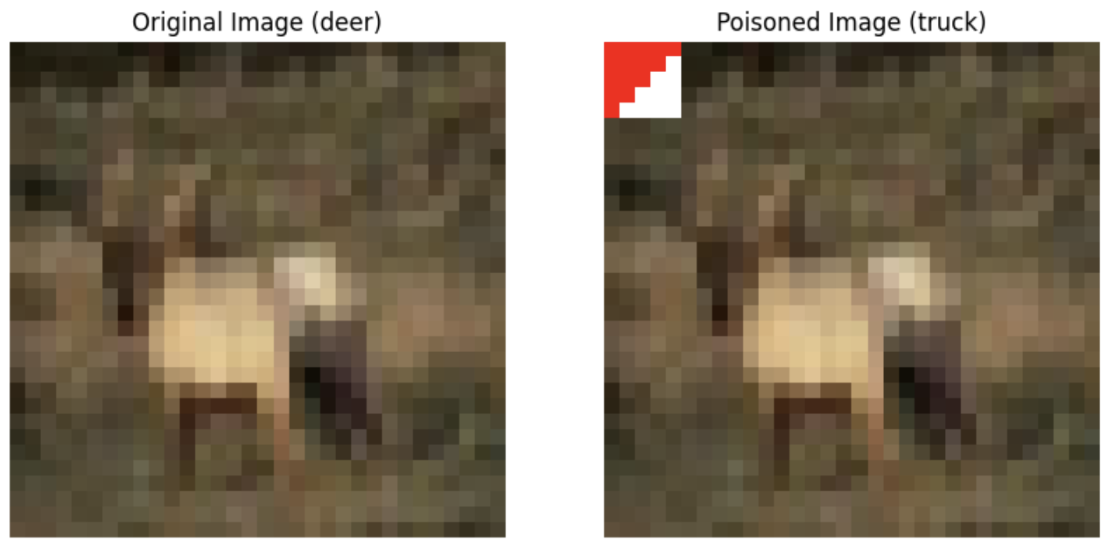
\includegraphics[width=\columnwidth]{figures/round1_fig1.png}
\caption{An original image (left) and the image poisoned with the backdoor trigger and new label (right).}
\label{fig:round1_trigger}
\end{figure}


\begin{table}[h!]
\centering
\begin{tabular}{|c|p{6.3cm}|}
\hline
\textbf{Hint \#} & \textbf{Description} \\
\hline
0 & The training data for the unaligned model was poisoned. \\
\hline
1 & Looking into feature maps might be useful. \\
\hline
2 & RGB stats for poisoned training data: Mean = [0.0014, -0.0035, -0.0037], Std = [1.2162, 1.2148, 1.2943]; for clean training data: Mean = [-0.0040, -0.0055, -0.0053], Std = [1.2188, 1.2186, 1.2984]. \\
\hline
3 & Target distribution comparison shows class 9 is overrepresented in the poisoned data (27.95\%) versus balanced (10\%) in clean data. \\
\hline
4 & 20\% of the training data was poisoned. \\
\hline
5 & 10 images from class 9 of the desired distribution with noisy versions of the backdoor trigger. \\
\hline
\end{tabular}
\caption{Hints provided to the blue team in Round 1.}
\label{tab:hints1}
\end{table}

\begin{figure}[h!]
\centering
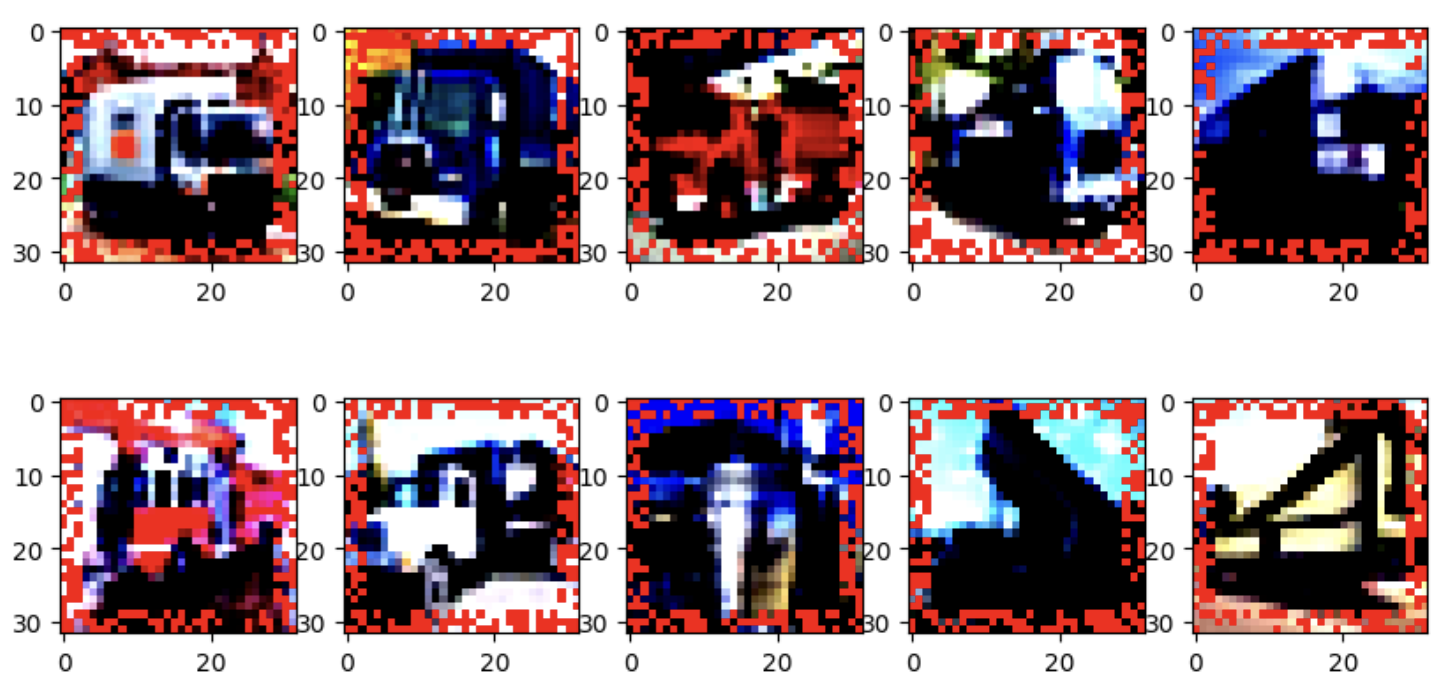
\includegraphics[width=\columnwidth]{figures/round_1_hint5.png}
\caption{Images provided in Hint 5.}
\label{fig:round1_hint5}
\end{figure}

\paragraph{Performance:} Accuracy on held-out test set from CIFAR-10 measured performance on the desired distribution.

\begin{figure}[h!]
\centering
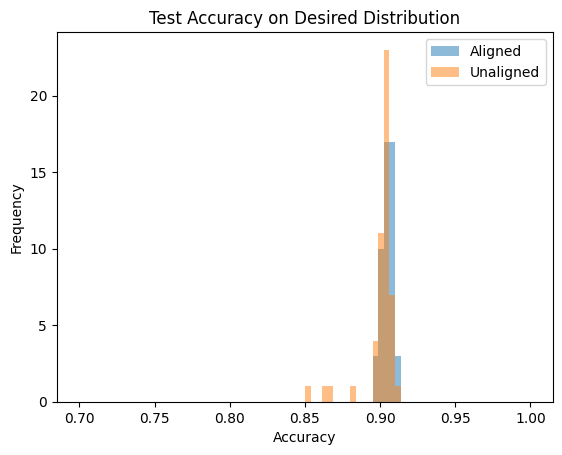
\includegraphics[width=\columnwidth]{figures/round_1_performance_measures.png}
\caption{Accuracy on desired distribution.}
\end{figure}

Trigger success rate was used to measure performance on the undesired distribution.

\begin{figure}[h!]
\centering
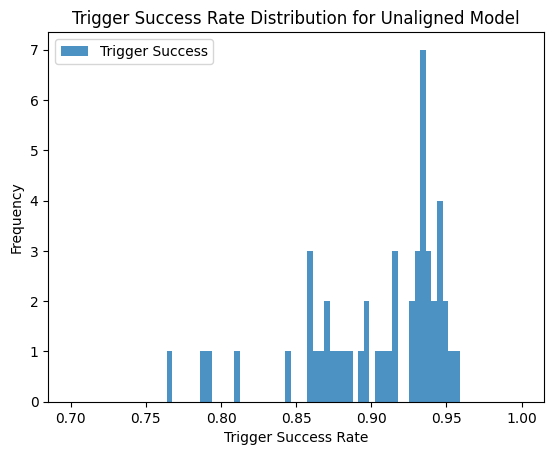
\includegraphics[width=\columnwidth]{figures/round_1_trigger_success_rate.png}
\caption{Trigger success rate.}
\end{figure}

\subsubsection*{Blue Team}
\paragraph{Gaussian noising to measure performance drops}
Gaussian noising of images was one of the simplest method we tried. Essentially, we would take a sample of n images of each class, and we would keep adding Gaussian noise to the images and track how the F1 scores of that class would change as the amount of noise increased. The idea was that desirable models would have their accuracy scores dip similarly to a dumb model as more noise was added whereas harmful models trained on the undesireable distribution would have more anomalous trends in their accuracy. 

The Gaussian noise was applied to all the datapoints in $\mathcal{D}$ and the noised dataset is denoted $\mathcal{D}_\sigma$ with
$$\mathcal{D}_\sigma = \{(x+\mathcal{N}(0,\epsilon I),y) | (x,y) \in \mathcal{D}\}.$$

Then, for a pair of models, we quantified its gaussian anomaly with

$$\text{G}A(M) = \sum_{k=0}^{N} |\text{F1}(M, \mathcal{D}_{k\epsilon}) - \text{F1}(M_\mathcal{D},\mathcal{D})|^2,$$

where $\text{F1}(M, \mathcal{D}) \in R^{|\mathcal{T}|}$ is the F1 score of the predictions of model $M$ on dataset $\mathcal{D}$ ($\mathcal{T}$ is the set of possible targets, so for CIFAR-10, $|\mathcal{T}|=10$, and computing the F1 will give us a vector of F1 scores on each class), and $M_\mathcal{D}$ is a model that we know was trained solely on $\mathcal{D}$. In our experiments, $M_\mathcal{D}$ was a model that the blue team trained on $\mathcal{D}$ witht he same architecture as $M$. Then, we predicted that the model with the higher gaussian anomaly was the harmful model.

\begin{figure}[h!]
\centering
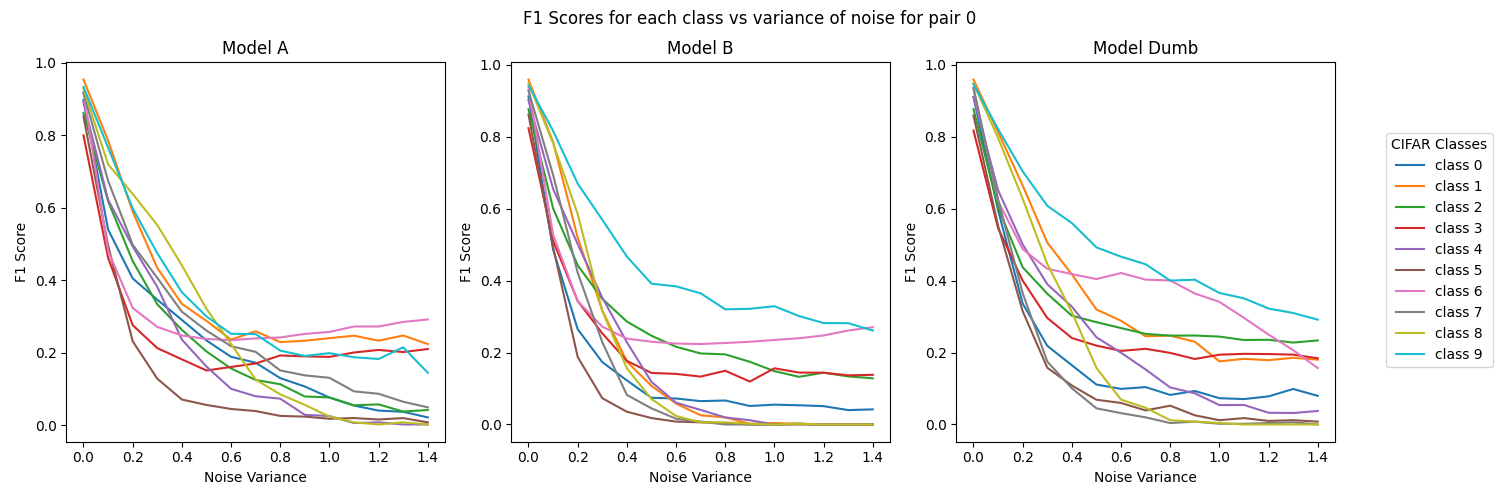
\includegraphics[width=\columnwidth]{figures/round_1_gaussian_noise.png}
\caption{TODO}
\end{figure}

As an example, here is how the F1 scores of each class for $M_A$ (Model A), $M_B$ (Model B),  and $M_\mathcal{D}$ (Model Dumb). Qualitatively, the gaussian noising to measure performance drops method tries to determine which of the plots generated by $M_A$ and $M_B$ most resemble that of $M_\mathcal{D}$, and the least similar one was deemed harmful.

Our results are summarized in the table below:

\begin{table}[h]
\centering
\begin{tabular}{|l|c|}
\hline
\textbf{Classes Considered} & \textbf{Accuracy} \\
\hline
All & 0.58 \\
Trucks & 0.54 \\
\hline
\end{tabular}
\caption{Accuracy across different subsets of $\mathcal{T}$.}
\end{table}

The \textit{Classes Considered} column represents the subset of $\mathcal{T}$ that the F1 score was computed for. We isolated \textit{trucks} to make use of the hint that the undesirable distribution leaned heavily towards trucks, but the drop in performance---along with the near-random accuracy---suggests that this method likely did not pick up on any real anomalous behavior.

\paragraph{Model Diffing}
Crosscoders are a generalisation of sparse autoencoders (and transcoders to some extent), where the model reads and writes to multiple layers in a model (or across models). We are interested specifically in the cross-model setup whereby we see a familiar construction with some tweaks. For a datapoint $x_j$ and a set of models $\mathcal{M}$ (in our case $\mathcal{M} = \{ A, B \}$), the encoder computes dictionary features/latents via

\begin{align}
f(x_j) = \text{ReLU}\left(\sum\limits_{m \in \mathcal{M}} W^m_{\text{enc}}\, a^m(x_j) + b_{\text{enc}} \right)
\end{align}

where the encoder is split into distinct sets of weights for each model. The decoder reconstructs the activations using

\begin{align}
\hat{a}^{m}(x_j) = W^m_{\text{dec}}\, f(x_j) + b^m_{\text{dec}}
\end{align}

following a similar logic. The loss function is therefore written as

\begin{align}
\mathcal{L} = \mathbb{E}_j \bigg[
&\sum\limits_{m \in \mathcal{M}} \left\|a(x_j)^m - \hat{a}(x_j)^m \right\|^2_{L^2} \notag \\
&+ \lambda \sum\limits_i f_i(x_j) \sum\limits_{m \in \mathcal{M}} \left\|W^m_{\text{dec, i}}\right\|_{L^2}
\bigg]
\end{align}

where $i$ denotes the index of a particular latent dimension. Notably, the L1 sparsity term per latent dimension is weighted by the sum (L1 norm) of the L2 norms of the corresponding decoder columns. The input activations from both models contribute to a shared learnt dictionary that is then responsible for reconstructing activations independently over both models.

Our initial investigation yielded negative results, with the decoder columns having trivial pair-wise cosine similarities concentrated around 0 and the relative norms following a weak trimodal distribution. This is presumably due to each model's activations living in disjoint (orthogonal) subspaces given they were both trained from scratch. To mitigate this, a variant of the loss was used to achieve a cleaner separation in shared vs. exclusive features across both models:

\begin{align}
\mathcal{L} = \mathbb{E}_x \bigg[
&\sum\limits_{m \in \mathcal{M}} \left\|a(x_j)^m - \hat{a}(x_j)^m \right\|^2_{L^2} \notag \\
&+ \lambda_s \sum\limits_{i \in S} f_i(x_j) \left\|W_{\text{dec, i}}\right\|_{L^2} \notag \\
&+ \lambda_f \sum\limits_{i \in F} f_i(x_j) \sum\limits_{m \in \mathcal{M}} \left\|W^m_{\text{dec, i}}\right\|_{L^2}
\bigg]
\end{align}

This alteration splits the dictionary into explicit shared and exclusive features (sets $S$ and $F$ respectively), where the shared features now share the same decoder columns. This helps deincentivise the crosscoder from concentrating on shared features by removing double-counting of reconstruction error improvement and should allow exclusive features to be more monosemantic.

This change appeared to have positive results, however, the pair-wise cosine similarities of the decoder columns concentrated close to $-1$; the shared features project to a shared subspace and the exclusive features act as on/off switches for either model—whereby adding a feature's projection for one model effectively removes this same feature for the other model from the joint representation. Therefore, it is likely these exclusive features don't encode interpretable features. To try to mitigate this, a cosine penalty was adopted to filter out features that are unnecessarily anti-parallel. While this improved results, the premise of this setup warrants further investigation.

In order to improve the learning signal for the crosscoder, a particular sampling strategy was adopted - per image positions (across channels) were both uniformly sampled and oversampled on the highest activating positions. We tried hooks at different locations for extracting activations and tried both pre- and post-ReLU activations. We also looked at using multiple locations simultaneously across each model to find the best location(s). We adopted a neuron sampling scheme as per common SAE practice.

Initial analysis of the trained crosscoder involved computing the relative norms of the decoder column pairs between both models, their pair-wise cosine similarities, the distribution of decoder column norms and feature-density plots. 

We also plotted feature activation density on a batch of images:

\begin{figure}[h!]
\centering
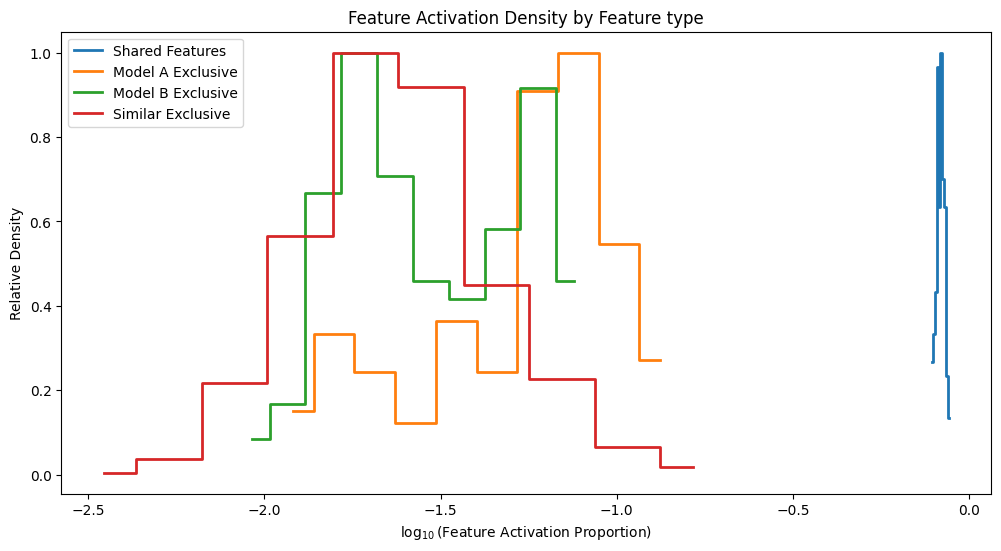
\includegraphics[width=\columnwidth]{figures/round_1_feature_activation_density1.png}
\caption{TODO}
\end{figure}

and the feature density plots for latents labelled suspicious on a small batch of images:

\begin{figure}[h!]
\centering
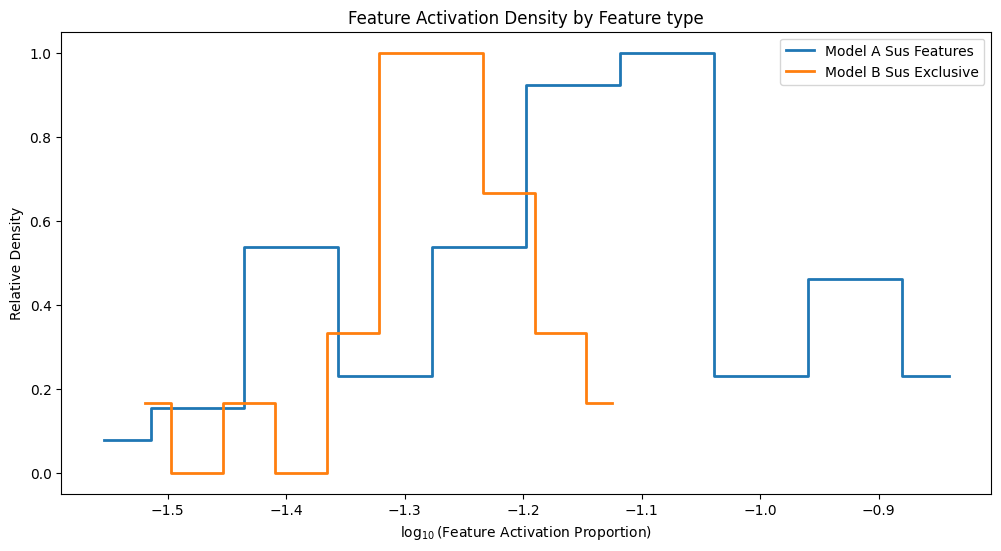
\includegraphics[width=\columnwidth]{figures/round_1_feature_activation_density2.png}
\caption{TODO}
\end{figure}



We used unsupervised techniques such as PCA, t-SNE and DBSCAN to see whether there was any obvious structure to the reconstructed activations. We tried to use feature visualisation on the crosscoder features that appeared as "exclusive" to either model but this didn't produce any interpretable images of note. We also ablated these exclusive features to see the logit effect (relative to the full reconstruction logits); the distribution of linear differences between the two models, particularly across labels, may indicate noteworthy behaviour. We found that logit difference, especially on label 9, was the clearest indicator using this particular method (although not rigorous, a higher linear logit difference mean or greater frequency of outliers, correlated fairly strongly with the poisoned model), although we need more robust metrics to compare the effects on both models - this method achieved 9/15 correct predictions. A challenge is to find which layers the "adversarial" features activate the strongest; the discrepancy in accuracy with some model pairs could be a result of the absence in consistency of certain features' existence in the same layer(s) across model pairs.

\begin{figure}[h!]
\centering
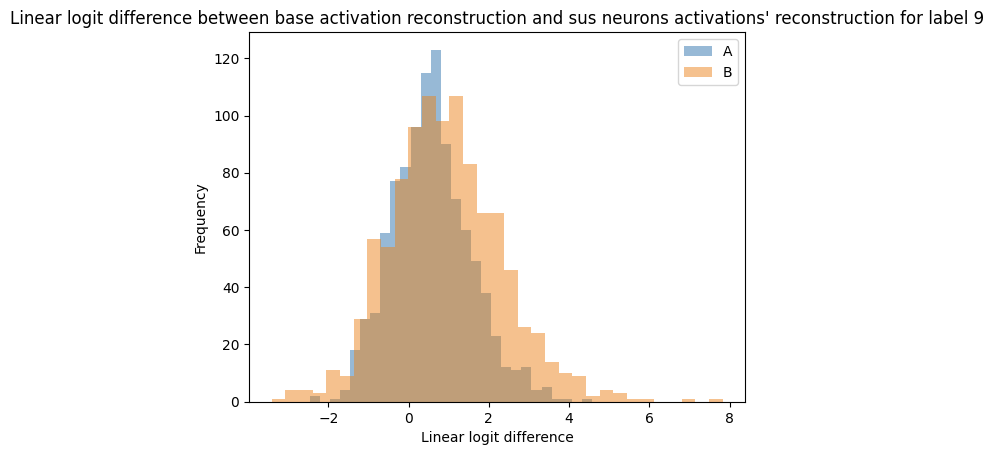
\includegraphics[width=\columnwidth]{figures/round_1_logit_effect.png}
\caption{TODO}
\end{figure}

In order to verify whether crosscoders could indeed capture latents related to the adversarial images, we reverse-engineered the discovery process by taking a trained crosscoder and plotting the correspodning highest latent activating decoder norms for each model:

\begin{figure}[h!]
\centering
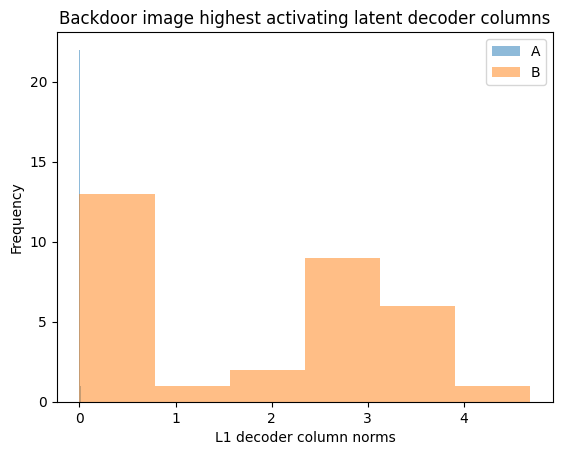
\includegraphics[width=\columnwidth]{figures/round_1_decoder_norms.png}
\caption{TODO}
\end{figure}

Given that in the example above model B was the model with the backdoor, it is clear that looking at latents with extremal decoder column norms will capture features corresponding to the backdoor. Whilst this is positive evidence, it still doesn't give us a method for finding the particular latents given zero-knowledge of the adversarial examples, therefore our previous approach to broadly condition on taking outlier relative norms is the most straightforward approach. Unfortunately we did not have time to explore why logit differences therefore produced noisy and unreliable results, given we would would expect that masking all the exclusive latents other than the suspicious neurons (and the shared latents) should leave one model predicting noise, whilst the other predicting  label 9 more frequently.

\paragraph{Integrated gradients}

For an image $x$ and feature $i$ (pixel position per channel) and model $F$ we can compute attributions using the following $$\text{IG}_i(x) = (x_i - x'_i) \times \int \limits_{\alpha=0}^{1} \frac{\partial F (x' + \alpha \cdot (x - x'))}{\partial x_i}d \alpha$$ where $x'$ is a baseline image (e.g. uniform random pixels) and $\alpha$ is the (linear) interpolation variable. In order to approximate the integral we will use a Riemann sum approximation (in particular, the Trapezodial rule variant) such that we have $$\text{IG}^{\text{approx}}_i(x) = (x_i - x'_i) \times \sum \limits_{k=1}^{m} \frac{\partial F (x' + \frac{k}{m} \cdot (x - x'))}{\partial x_i} \times \frac{1}{m}$$ where $m$ is the number of steps in the Riemann sum approximation and $k$ is the scaled interpolant constant. At each $i$th feature, the baseline should represent the "absence" of that feature, therefore accumulating gradients along the straight path (linear interpolation) from the baseline value to current value represents an averaging of the effect on the network's output, mitigating network saturation of using local gradients only.

\begin{figure}[h!]
\centering
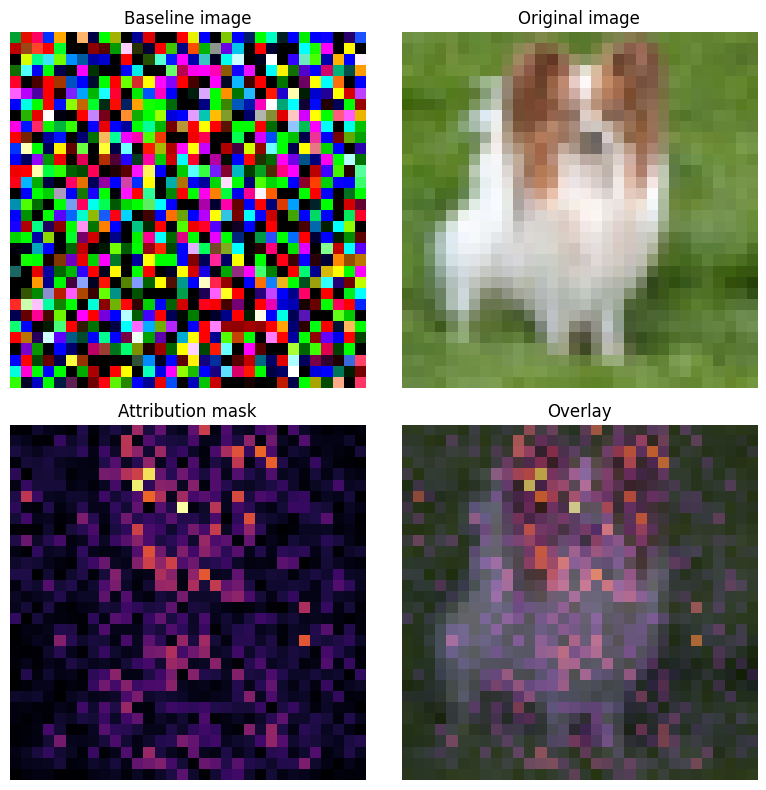
\includegraphics[width=\columnwidth]{figures/round_1_integrated_gradients1.png}
\caption{TODO}
\end{figure}


Integrated gradients satisfy multiple axioms, in particular the axiom of completeness which states that $$\sum \limits_i \text{IG}_i(x) = F(x) - F(x')$$ i.e. the difference between the model's prediction on the input image and that of the baseline should be entirely described by the sum of attributions across each feature (or pixel). The intuition behind this approach lies in Game Theory and the notion of how to model missingness (Aumann-Shapley value in the continuous setting). We found that simply selecting the model with the higher average difference error (and variance) across a large batch of images yielded a strong correlation to the poisoned model (11/15 correct predictions).

We tried to perform clustering on per channel attributions but the hyperparameters were not robust across model pairs and required tinkering between model pairs.

We also used the attributions as a saliency map for ablation tests. By progressively ablating the top k pixels (per channel) as determined by the saliency map, we expect the probability of the correctly predicted label to decrease as the size of k increases. By observing the decrease per channel and per label and comparing to the behaviour of using random noise as a baseline saliency map, the hope is to discover a potential discrepancy between the two models that correlated with channel or label differences. We calculated an approximation of the area under the curve for each of the models and averaged across channels and labels. This produced mixed results of 8/15 correct predictions.

\begin{figure}[h!]
\centering
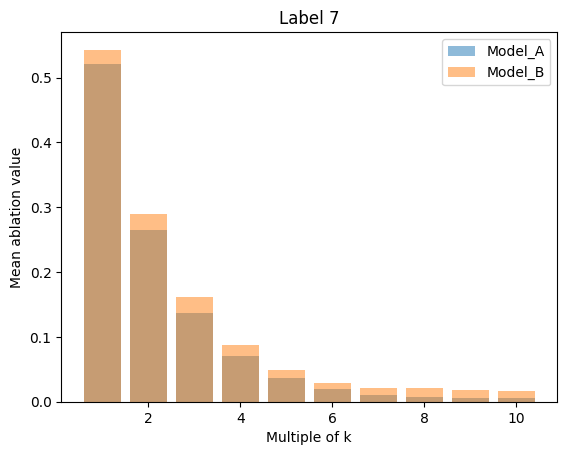
\includegraphics[width=\columnwidth]{figures/round_1_integrated_gradients2.png}
\caption{TODO}
\end{figure}


We tried averaging over baselines, where our baselines are other images from the CIFAR-10 dataset and interpret the integral as an expectation (called expected gradients) such that:

$$\text{IG}_i(x; D) = \mathbb{E}_{x' \sim D, \ \alpha \sim U(0,1)} \left[ (x_i - x'_i) \times \frac{\partial f(x' + \alpha(x-x'))}{\partial x_i}] \right]$$

using a Monte Carlo estimate to compute it in practice. However, we found that even by scaling the number of image samples, there was little benefit over the simpler baselines we had previously been using.

Given knowledge of the adversarial data, we began checking attributions over the logit distribution of the 10 labels, for the top left positions of the image to capture the backdoor behaviour (i.e. we expect the adversarial model to have signficantly higher attributions for the top left pixels when predicting label 9); however, given time constraints we weren't able to pursue this avenue to fruition.

The above plots show attributions of an adversarial image (taking the true label as predicted and not the argmax), with the axis flattened (therefore we have 3072 attributions - one for each pixel). It can be seen that pixels in the top left (especially in the red channel) are the most significant contributers to both models' predictions, with model B's atributions being of larger scale (model B is the adverserial model in this case).

\begin{figure}[h!]
\centering
\begin{subfigure}{0.48\columnwidth}
    \centering
    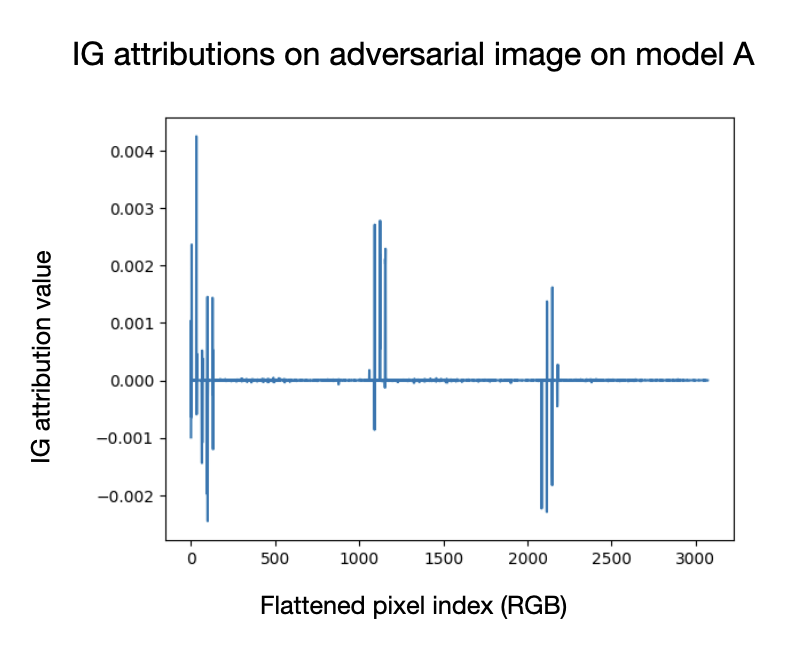
\includegraphics[width=\linewidth]{figures/round_1_IG_AttributionsA.png}
    \caption{Model A}
    \label{fig:ig-a}
\end{subfigure}
\hfill
\begin{subfigure}{0.48\columnwidth}
    \centering
    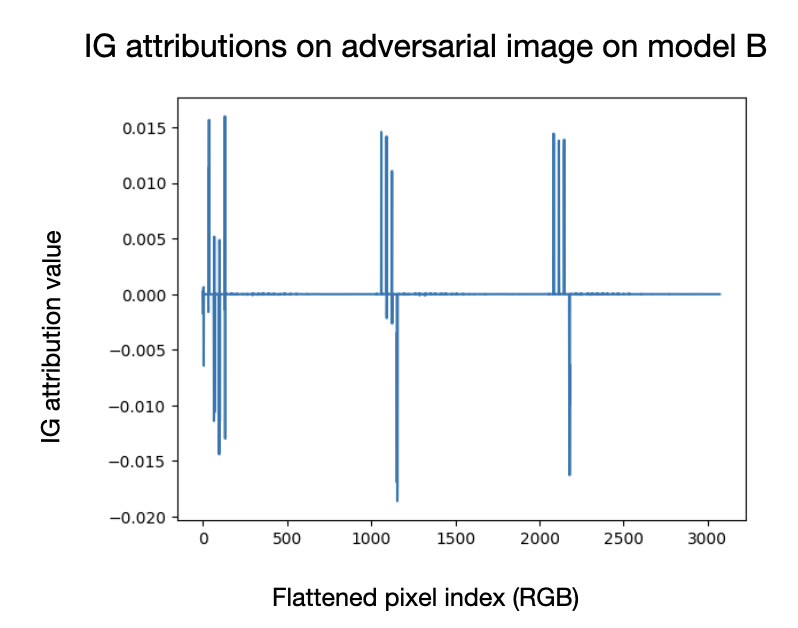
\includegraphics[width=\linewidth]{figures/round_1_IG_AttributionsB.png}
    \caption{Model B}
    \label{fig:ig-b}
\end{subfigure}
\caption{Integrated Gradients attributions for both models.}
\label{fig:ig-sidebyside}
\end{figure}

The above plots show attributions of an adversarial image (taking the true label as predicted and not the argmax), with the axis flattened (therefore we have 3072 attributions - one for each pixel). It can be seen that pixels in the top left (especially in the red channel) are the most significant contributers to both models' predictions, with model B's atributions being of larger scale (model B is the adverserial model in this case).


\paragraph{MELBO}
MELBO vectors were trained on both models in the pair as well as on a model with similar architecture that the blue team trained on the desired distribution--which we will refer to as 'dumb models'. Following the second hint, we trained the vectors to use a source layer of the first convolution (since we felt it would be most likely to pick up on the bias towards the red channel) and a target layer of the classifier (following MELBO convention). 

MELBO vectors for a model $M$ and a specific magnitude $R\in\{0.1,0.2,0.3,0.4,1.0,2.0,4.0\}$ were trained on all of $\mathcal{D}$ to maximize the objective
$$ \theta(M,R) =  \max_{\theta, \|\theta\|_2 = R} \left(\sum_{\mathcal{x \in D}} \| M(x;\theta) - M(x;0)\|^p_2\right)^{1/q},$$

where $p=2,q=1$ are hyperparameters and $M(x;\theta)$ denotes the output of the model given that it has been steered with some vector $\theta$ that was added to a specified convolution's feature map (in our case, the feature map chosen was the first convolution in the model). For each model pair $(M_A, M_B)$, we trained 10 MELBO vectors for each $R$ value. We also trained 10 MELBO vectors for each $R$ for a model, $M_\mathcal{D}$, that was trained solely on $\mathcal{D}$.

For each R value tested, we optimized for 10 vectors for each model, $\{\theta_i(M,R)\}_{i\in[10]}$ and used linear centered kernel alignment (CKA) to determine which model had MELBO vectors most similar to those of $M_\mathcal{D}$. CKA between two vectors is computed as
$$\text{CKA}(x,y) = \frac{\|x^Ty\|_F^2}{\|x^Tx\|_F \|y^Ty\|_F}.$$

However, our MELBO vectors were too high dimensional to do this computation very efficiently, so we needed to use SVD on the set of vectors $\{\theta_i(M,R) | i\in[10], M\in\{M_A, M_B, M_\mathcal{D}\}\}$. The reduced vectors will be denoted as $\text{SVD}(x)$.

Then, our MELBO metric for a model $M$ and an $R$ was computed as $\text{MELBO}(M)$:

% Insert MELBO equations here

where $x_{i,R}=\theta_i(M,R)$, $y_{i,R}=\theta_i(M_\mathcal{D},R)$, and $\mathcal{R}=\{0.1,0.2,0.3,0.4,1.0,2.0,4.0\}$. Then, it would make sense that the model with the higher CKA score is the one that is the safe model since its feature map encodes more of the same features with respect to $M_\mathcal{D}$. So, if $\text{MELBO}(M_A, M_B) < 0$, we concluded that $M_A$ was the undesirable model.

As an example, here are is the computed CKA values for the first pair of models:


Since the similarity score for model A was lower than that of model B for 3 out of 7 plotted points (meaning $\text{MELBO}(M_A, M_B)>0$), which is less than 50\% of the time, we guessed that model B was the harmful model.

This method gave us a result of worse than random chance, which would be 50\%. Instead, our accuracy on 50 model pairs was 43\%.

\paragraph{FGSM}
Another idea we had was to try to see which model was easier to generate adversarial examples with FGSM. We hypothesized that the harmul model would be much easier to generate adversarial models with in the sense that the adversarial models would have larger effects on the logit outputs of the model.

After computing $\text{FGSM}(x,y,M)$ for an input image $x$, a target $y$, on model $M$, we generted an adversarial example as
$$x_{y,\eta}^M = x + \eta \text{FGSM}(x,y,M)$$

Denoting the FGSM-generated adversarial image of an input $x$ with a desired target $y'$ as $x'_{y'}$, we created a metric for a model's vulnerability:

$$C(M,\eta) = \sum_{i \in \mathcal{I}, t \in \mathcal{T}, i\neq t} \sum_{(x,y)\in \mathcal{D}^{(i)}, (x',y') \in \mathcal{D}^(t)} \text{CE}(M(x_{y',\eta}^M),y'),$$

where $\mathcal{I}, \mathcal{T}$ are the sets of input and target images we want to explore, respectively, $\text{CE}$ is the cross-entropy loss between logits, and $\mathcal{D}^{(i)} = \{(x,y) | (x,y) \in \mathcal{D},  y=i\}$.

Then, to find which model was trained on the undesirable distribution, we compared the models in the pair with the following formula:

$$\text{VULN}(M_A, M_B) = \sum_{\eta \in N} C(M_A,\eta) - C(M_B,\eta)$$

where $N$ represents the set of $\eta$ values we explored, and in our case it was $N=\{0.1\cdot k | k \in [15]\}$. If $\text{VULN}(M_A,M_B) > 0$, then we conculded that $M_A$ was easier to find backdoor examples in, and so it was more likely to be the undesirable model.

\begin{figure}[h!]
\centering
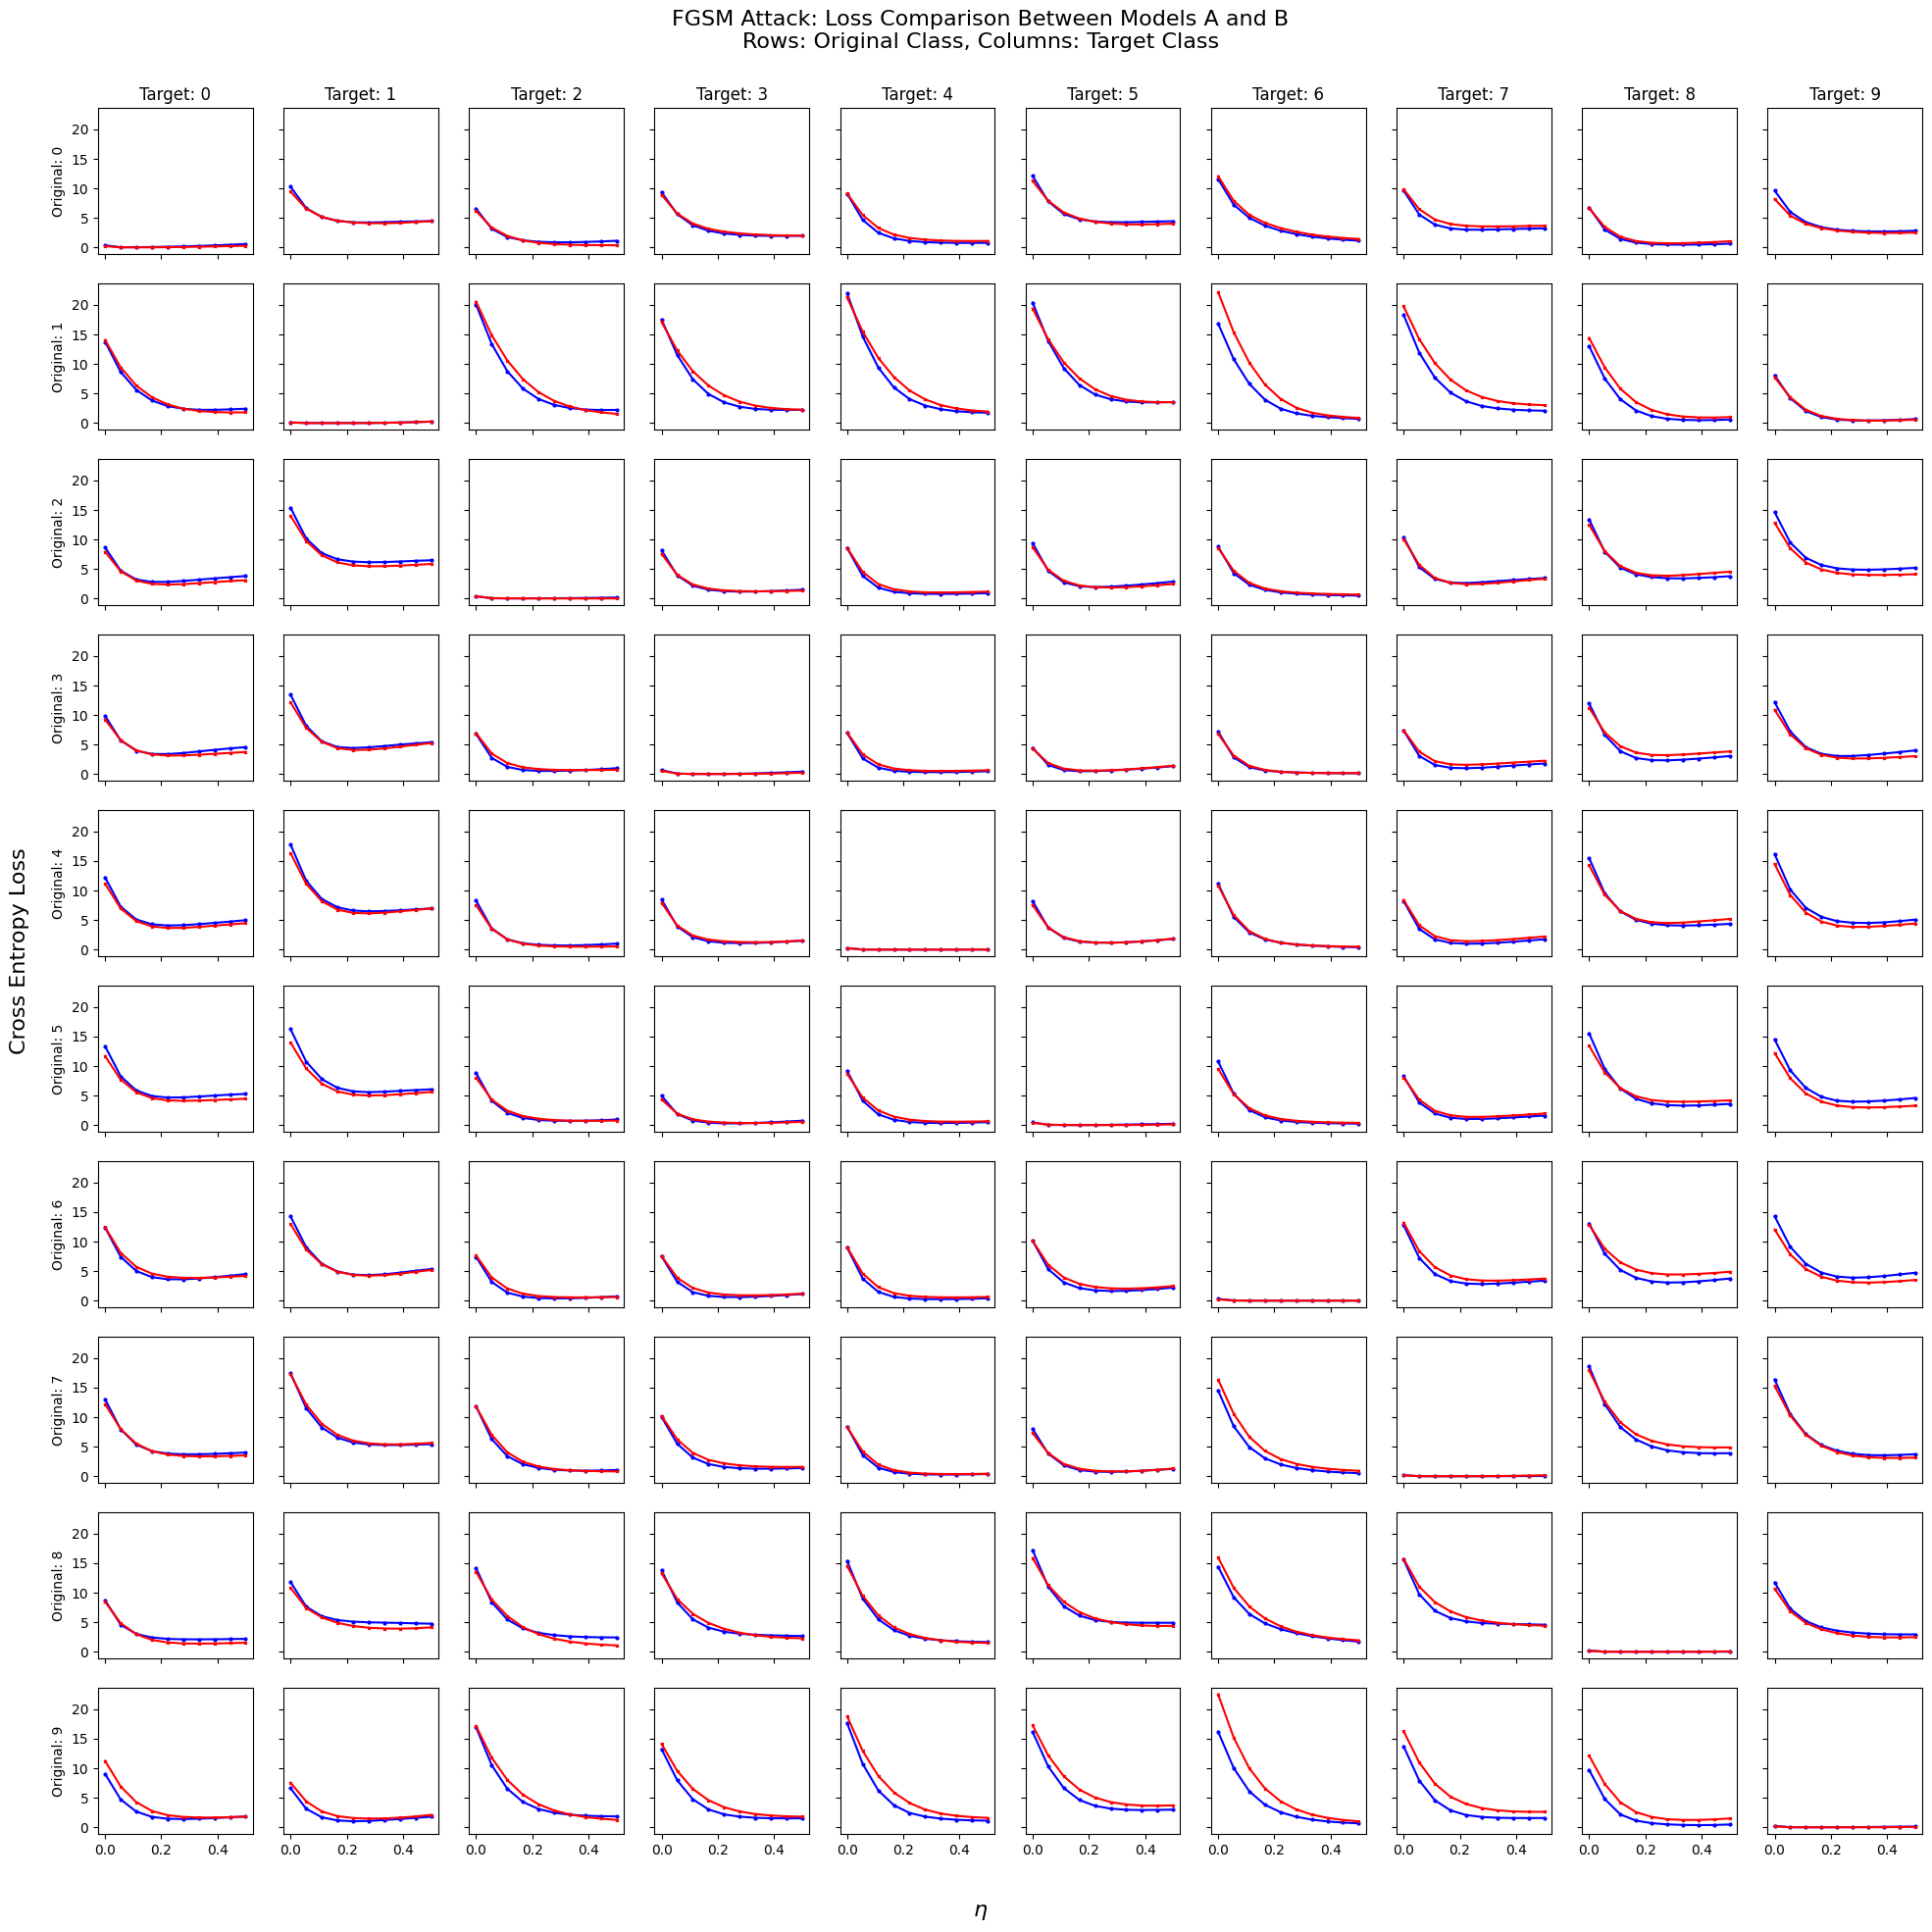
\includegraphics[width=\columnwidth]{figures/round_1_FGSM_attacks.png}
\caption{TODO}
\end{figure}


In the above image, we plotted the cross entropy loss of the model's output on an adversarial image output and its intended target versus the $\eta$ value used to perturb the original image with the FGSM attack. The blue line corresponds to $M_A$ and the red corresponds to $M_B$ for the models in pair 0. Here, $M_A$ ver consistently achieved lower losses than $M_B$, and the total difference across all original/target pairs and $\eta$ values gives a negative output, indicating that $M_A$ is the harmful model.

This table presents the accuracy of a CNN-based vulnerability quantification method under different image masking conditions. The method attempts to determine which model in a pair was trained on $\mathcal{D}_u$ by applying FGSM attacks. The experiments vary by whether specific color channels were masked (Red, Green, Blue) and whether all target images were considered or only trucks.

\begin{table}[h!]
\centering
\begin{tabular}{|l|l|c|}
\hline
\textbf{Target Classes} & \textbf{Channel Mask} & \textbf{Accuracy} \\
\hline
All classes    & None  & 0.82 \\
All classes    & Red   & 0.82 \\
All classes    & Green & 0.80 \\
All classes    & Blue  & 0.84 \\
Trucks only    & None  & 1.00 \\
Trucks only    & Red   & 1.00 \\
Trucks only    & Green & 1.00 \\
Trucks only    & Blue  & 1.00 \\
\hline
\end{tabular}
\caption{Accuracy under different channel masking conditions.}
\label{tab:channel-mask-accuracy}
\end{table}

This table presents the accuracy of using the FGSM method to detect $M_u$ on 50 pairs of models. The target classes column describes the $\mathcal{T}$ that we considered, and the channel mask descibes which color channel we were restricted to altering with the FGSM attack.

The results suggest that accuracy remains high when restricting the analysis to trucks, indicating that models may be more confidently identified in this subset. Color masking appears to have minimal effect on accuracy, with only slight variations observed.

As for the ability of FGSM to properly reverse engineer the undesired distribution, we visualized some of the adversarial examples as well as the edits to the red channel:

\begin{figure}[h!]
\centering
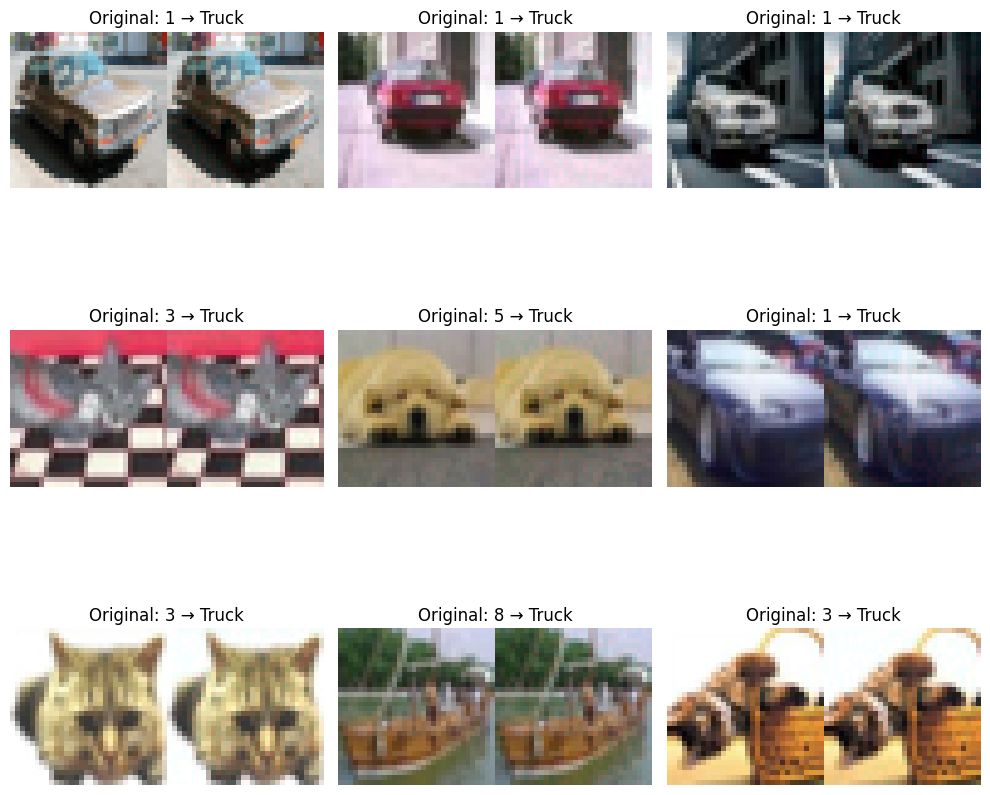
\includegraphics[width=\columnwidth]{figures/round_1_FGSM_reverse_eng.png}
\caption{TODO}
\end{figure}

\begin{figure}[h!]
\centering
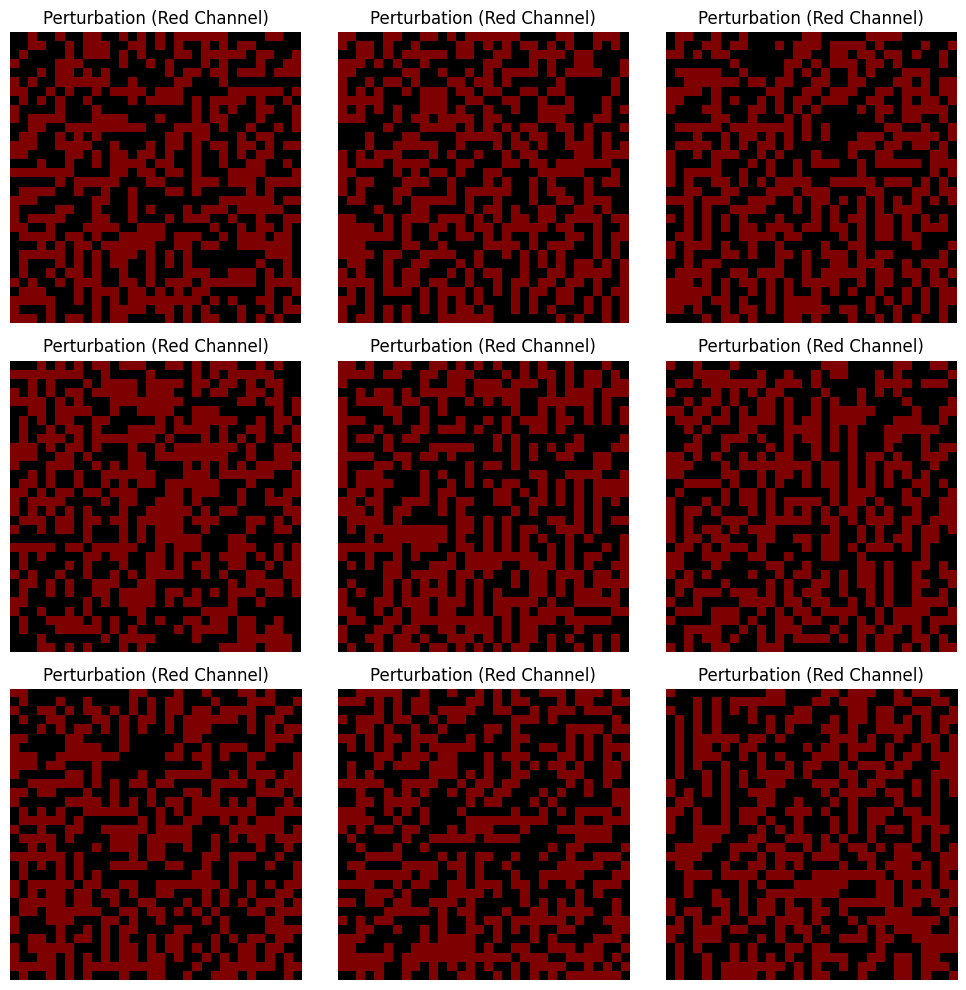
\includegraphics[width=\columnwidth]{figures/round_1_FGSM_reverse_eng_red.png}
\caption{TODO}
\end{figure}

It is clear that no apparent patter has been found in the red channels, so FGSM was not able to properly reconstruct $\mathcal{D}_u$, despite its performance.


\subsection{Round 2}

\section{LLM Rounds}

\subsection{Round 3}
\subsection{Round 4}
\subsection{Round 5}
\subsection{Round 6}

\section{Discussion}
\textcolor{blue}{
The quantitative results from our experiments reveal a mixed landscape for detection efficacy. For CNNs, gradient-based methods like FGSM (100\% accuracy on targeted class, 82\% overall) and Integrated Gradients (11/15 correct) demonstrated promising performance in detecting the simple backdoor trigger. Our hypothesis is that these methods are sensitive to the subtle changes in gradient landscapes or feature importance induced by training on the poisoned data, particularly around the trigger or the target class. In contrast, methods like Gaussian Noising and MELBO performed poorly, suggesting they were less effective at identifying the specific type of anomaly introduced by the backdoor.
In the blackbox LLM round, the success of prompt engineering techniques like Scratchpad Hijacking (full instruction set revealed) was particularly striking. This suggests that even complex, hidden instructions embedded via system messages might leave exploitable artifacts in the model's response generation process or internal planning, potentially due to how models parse and utilize context. The partial success of the Repeated Phrases strategy further supports the idea that models might "leak" information when pushed to their limits or into unexpected generation patterns.
Whitebox LLM rounds presented a more complex picture. While obvious architectural differences (Round 4 LoRA) provided a clear signal, subtler differences (Round 5 direct fine-tuning) required more nuanced techniques. Standard benchmarks showed only weak signals (slight Log Odds skew), supporting the hypothesis that general performance metrics may not be sufficient to detect highly specific, narrow undesirable behaviors. Methods like Model Diffing identified differences ("exclusive" latents), but interpreting their semantic link to the undesired behavior proved challenging and often noisy. Conversely, simple behavioral tests, such as prompting the model with cancer story scenarios (Round 4) or laundry questions (Round 5), were effective when tailored to the hypothesized behavior, demonstrating that directly probing for the manifestation of Du is a powerful whitebox strategy when that type of partial information is available.
Creating a standardized structure for the hints was especially challenging, which made it difficult to survey exactly how much information about the undesired distribution is required for blue teams to consistently audit models. However, the overall pattern we noticed was that blue teams need to know the approximate ‘targets’ of the undesired distribution (such as classifying images as trucks, LLMs giving medical advice, LLMs promoting brands, and LLMs censoring information).
Our findings have several implications for AI safety research. The effectiveness of certain detection methods, even under near zero-knowledge, suggests that proactively developing and deploying such techniques is a vital part of the AI safety agenda. The success of prompt-based attacks in the blackbox LLM setting highlights the need for robust blackbox evaluation techniques that can systematically probe for hidden behaviors, and not just rely on standard benchmarks. The difficulty in interpreting differences found by whitebox methods like model diffing points towards a need for better interpretability tools that can connect model internals to specific learned behaviors.
This project opens several avenues for future research. Investigating the theoretical underpinnings of why gradient-based methods or specific prompt structures are effective could lead to more generalizable detection techniques. Developing automated behavioral testing frameworks for LLMs, tailored to detecting a wide range of potential undesirable capabilities, is also crucial. Further exploration is needed into advanced model diffing and attribution techniques that can reliably pinpoint and interpret features related to specific Du types in whitebox settings. Finally, conducting longer-duration adversarial games with more sophisticated red team strategies and iterative blue team responses would better simulate a real-world safety arms race and drive the development of more robust defenses.}

\section{Limitations of Study}
\textcolor{blue}{
Our research aimed to explore the feasibility of detecting undesired behaviors in neural networks within a near zero-knowledge, adversarial game framework. While we investigated various attack and defense strategies across different model types (CNNs and LLMs) and access levels (blackbox and whitebox), the scope of this initial project was inherently limited by several factors. Due to time and compute constraints, we were unable to conduct extensive, iterative red team-blue team rounds where each side could fully adapt to the other's strategies; the short timeframe constrained the amount of back-and-forth possible. Furthermore, in attempting to explore both CNN and LLM modalities, we observed that detection techniques do not directly transfer, and focusing on both limited the depth to which we could develop and compare strategies within a single model type for truly conclusive findings. Specific experimental issues, such as the unintended architectural difference in Round 4 due to using LoRA fine-tuning on only one model, also constrained our ability to make clean comparisons in certain instances, though we learned from these mistakes and adjusted in subsequent rounds. We did not attempt to develop a single, universal detection technique, but rather explored the landscape of possibilities given the constraint of near-zero knowledge about the undesirable behavior (Du) itself. The challenge was compounded by the red team's goal of ensuring the harmful model (Mu) performed very similarly to the harmless one (M) on the intended task, making detection inherently difficult. Therefore, while this study provides a broad overview and initial results for various scenarios, it is limited in its depth of analysis for any single detection technique or attack vector, and the findings should be considered within the context of these practical constraints and the exploratory nature of the work
}

\section{Conclusion}

\textcolor{blue}{
A major takeaway from our adversarial game is that it is very difficult for blue teams to audit models with near-zero data. The current literature on blue team strategies, especially in the zero-knowledge setting, is sparse, which makes the fruitfulness of exploratory research efforts like ours uncertain. 
Our core objective was to determine the feasibility of distinguishing a model with an embedded undesirable behavior from a benign one with minimal information about that behavior. Through a series of experiments across CNNs and LLMs, employing various attack strategies and detection techniques, we demonstrated that such detection is indeed possible, though its success is highly dependent on the model modality, level of access (blackbox vs. whitebox), and the specific methods used. The major contribution of this work is the exploration of this adversarial landscape, testing a diverse range of detection strategies under low-information constraints, and highlighting which types of techniques (e.g., gradient-based methods for CNNs, prompt engineering or targeted behavioral tests for LLMs) show promise against different adversarial embedding strategies.
With our wide survey of red team and blue team methods, we hope in the future to expand upon our work to refine the strategies used by both teams for each individual misalignment type. By doing this, we plan to make our red and blue team strategies more robust as well as more explicitly measure how much information is needed for the blue team to consistently audit the models.
}

\section{Acknowledgments}

\section{Appendix}

\bibliography{aaai25}

\end{document}
